\chapter{Robotic Manipulator Platform}
Given the problem space, a real-world and cooresponding simulated environment was created as a platform to train and test reinforcement learning algorithms for the neuro-symbolic architecture described in this paper and general reinforcement learning algorithms involving robotic manipulators.
The physical hardware used for this robotic manipulator is based on an open-source hardware design[CITATION], with modifications made to reduce cost while maintaining performance.
The cooresponding simulation and control of the manipulator was developed using the ROS2 middleware suite and nd Gazebo simulation enviroment enabling a flexible and reproducable setup for training, validating, and deploying algorithms.

\section{Robotic Manipulator Hardware}  \label{se:robotic_manipulator_hardware}
The physical hardware used to test the algorithms is made up of a 6-axis robot arm communicating over serial (UART) with a PC running the algorithms in a ROS2 Jazzy workspace.
The rigid components of the arm including gears and structural pieces are made of 3D-printed Polylactic Acid (PLA).
The robotic arm uses stepper motors, belts, and pulleys to articluate the 6 joints. 
The first 5 joints (J1 to J5) use bipolar NEMA 17 stepper motors, while the last joint J6, responsible for manipulating the end effector, uses a bipolar NEMA 8 stepper motor.
The belts and pulleys are "off-the-shelf" GT2 timing belts and pulleys of varying sizes, used to the torque applied to each joint (belts and pulleys connect every motor to a joint with the exception of J6).
Ball and shunt bearings of verious sizes are also used to reduce friction in the joints.

The electronic hardware is controlled by an ATmega328p microcontoller and 6 A4988 stepper motor drivers originally setup for controlling the stepper motors of a 3D-Printer.
Custom firmware was written for the microcontroller to run the 6 stepper motor drivers simultaineously with a serial (UART) inturrupt to recieve control commands from the host PC. 
\begin{figure}
	\centering
  \begin{tikzpicture}

    \node[draw,
      minimum width=2cm,
      minimum height=1.2cm,
      ] (input) at (0,0){$ROS2$};

    \node[draw,
      minimum width=2cm,
      minimum height=1.2cm,
      right=1.5cm of input
      ] (sum) {$\mu C$};

    \node[draw,
      align=center,
      minimum width=2cm,
      minimum height=1.2cm,
      right=1cm of sum 
      ]  (controller) {$Motor$\\$Drivers$};

    \node[draw,
      minimum width=2cm,
      minimum height=1.2cm,
      right=1cm of controller 
      ]  (plant) {$Robot$};

    \node[draw,
      minimum width=2cm,
      minimum height=1.2cm,
      right=1cm of plant
      ]  (encoder) {$Encoders$};

    \node[draw=none, right=1.5cm of encoder] (output) {$y$};

    \draw[->] (input.east) -- (sum.west) node[midway, above]{\tiny{$UART$}};
    \draw[->] (sum.east) -- (controller.west) node[midway, above]{$u$};
    \draw[->] (controller.east) -- (plant.west);
    \draw[->] (plant.east) -- (encoder.west);
    \draw[->] (encoder.east) -- (output.west);
    \draw[->] (output.center) ++(-1,0) |- ++(0,-1.25) -| (sum.south) node[midway, below]{};

  \end{tikzpicture}\\
	\caption{Robot servo feedback system.} 
\end{figure}


\subsection{Inverse Kinematics} \label{ss:inverse_kinematics}

\subsection{Motor Control} \label{ss:motor_control}
Bipolar stepper motors are used to move the joints of the robot, choosen for their low cost and wide availability. Stepper motors have 

A hobbiest 3D-printer stepper motor controller with custom firmware was used to reduce cost.
\begin{figure}[htb]
  \centering
  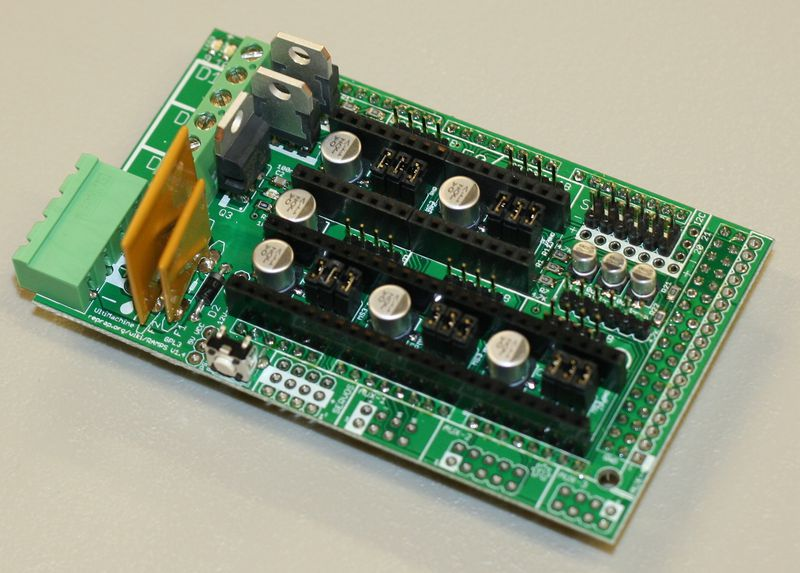
\includegraphics[scale=0.2]{RAMPS}
  \caption{RAMPS board}
  \label{fig:ramps}
\end{figure}

\subsection{Communication} \label{ss:communication}
Communication is done over a USB-UART connection, sending ROS2 position commands to a ATmega328p microcontroller used to process the position requests and update the joint positions.


\section{Robotic Manipulator Software} \label{se:virtual_overview}
The environment consists of the same six axis robot arm described in the previous section set up in the Gazebo Robotic Simulator (using a ROS Universal Robot Description File and Gazebo Simulation Description File).
Within the arm's working envelop various basic 3-D shapes (i.e. spheres, cubes, cylinders, etc.) are present.

The Robot Operating System is a middleware suite used for robot software development.
ROS workspaces consist of packages that interface with ROS libraries. 
\subsection{Robot Description} \label{ss:description_package}
The \texttt{arm\_description} package is a ROS package that contains various files used to describe the physcial characteristics of the robot including its visual, collision, control, and forward kinematics.

The six-axis robotic arm model deployed in this package is a slightly modified version of an open source six-axis robot design with modfications made to some of the pulleys and end-effector design. The robot arm is made up of six joints (J1-J6) all described as revolute joints in the \texttt{arm\_description}'s Universal Robot Description File (\texttt{.urdf}). Meshes for rendering the robot imported as \texttt{.stl} files and the meshes for collision areas are described by COLLADA (\texttt{.dae}) files. These meshes are linked together in the URDF in a kinematic chain to form the robotic arm manipulator.
Control of the robot is accomplished through the ROS Jazzy control package.
\subsection{Controllers}

\subsection{Hardware Interface}

\section{Reinforcement Learning Environment}
